% Slide 1: Introduction to Control Units
\begin{frame}
    \frametitle{Introduction to Control Units}
    \begin{itemize}
        \item The control unit directs CPU operations and generates control signals to execute instructions.
        \item Types of control units:
            \begin{itemize}
                \item \textbf{Unpipelined Hardwired Control Unit} (Von Neumann-style): Control signals generated directly by hardware.
                \item \textbf{Microprogrammed Control Unit} (Wilkes-style): Control signals generated by stored microinstructions.
                \item \textbf{Pipelined Hardwired Control Unit}: Adds pipeline stages for improved performance.
            \end{itemize}
        \item They aim to generate control signals,
        but they differ in implementation and use cases.
    \end{itemize}
    \note{
        This slide introduces students to the idea that control units
        play a critical role in CPU operation by generating the signals
        needed for instruction execution. We'll examine the characteristics,
        pros, and cons of two major types: unpipelined hardwired and microprogrammed units.
    }
\end{frame}

% Slide 2: Unpipelined Hardwired Control Unit
\begin{frame}
    \frametitle{Unpipelined Hardwired Control Unit}
    \begin{itemize}
        \item \textbf{Control Signal Generation}: Based on combinational logic from instruction and status bits.
        \item \textbf{Finite State Machine (FSM)}: Maps control signals to FSM states.
        \item \textbf{Direct Control}: Instructions directly trigger specific control signals through hardware.
    \end{itemize}
    \note{
        Hardwired control units generate control signals through combinational circuits,
        with each instruction mapped to specific signals.
        This approach is faster but less adaptable, making it suitable for RISC.
        Introducing the FSM concept here gives a high-level overview
        of states corresponding to control signals.
    }
\end{frame}

% Slide 3: Advantages of Hardwired Control Units
\begin{frame}
    \frametitle{Advantages of Hardwired Control Units}
    \begin{itemize}
        \item \textbf{Speed}: Faster execution due to direct signal generation.
        \item \textbf{Simplicity for Simple ISAs}: Suitable for RISC, where a simpler instruction set matches well with hardwired control.
        \item \textbf{Lower Latency}: Minimal delay since signals do not need to be fetched from memory.
    \end{itemize}
    \note{
        The speed of hardwired control units is a key advantage,
        as control signals are generated without the memory fetch
        delay seen in microprogrammed units.
        This makes them ideal for simpler, RISC-based architectures,
        which rely on rapid instruction processing.
    }
\end{frame}


% Slide 4: Disadvantages of Hardwired Control Units
\begin{frame}
    \frametitle{Disadvantages of Hardwired Control Units}
    \begin{itemize}
        \item \textbf{Inflexibility}: Modifications require hardware changes.
        \item \textbf{Design Complexity}: Complex to design for extensive instruction sets,
        such as CISC.
    \end{itemize}
    \note{
        Hardwired units lack flexibility;
        hardware updates are needed to add new instructions.
        This is particularly challenging for complex instruction set architectures,
        where the breadth of instructions demands more intricate control circuitry.
    }
\end{frame}


% Slide 5: Microprogrammed Control Unit
\begin{frame}
    \frametitle{Microprogrammed Control Unit}
    \begin{itemize}
        \item \textbf{Control Signals}: Generated through a stored microprogram.
        \item \textbf{Instruction}: Each machine instruction is broken into smaller steps called microinstructions.
        \item \textbf{Micro-instructions $\mu I$}: Set of data and resource independent micro-operations that can be executed in one clock cycle.
        \item \textbf{Micro-operations $\mu O$}: Control signals for the data flow in the processor.
    \end{itemize}
    \note{
        The microprogrammed control unit uses a microprogram—a sequence of microinstructions stored in
        memory—to generate control signals. Each high-level instruction is implemented as
        a series of micro-instructions. This unit is advantageous for handling complex
        instructions because it's easier to update and modify through changes to the microprogram,
        rather than requiring hardware changes.
    }
\end{frame}

% Slide 6: Microprogrammed Control Unit Components
\begin{frame}[fragile]
    \frametitle{Microprogrammed Control Unit Components}
    \begin{columns}
        \column{0.5\textwidth}
        \begin{figure}
            \centering
            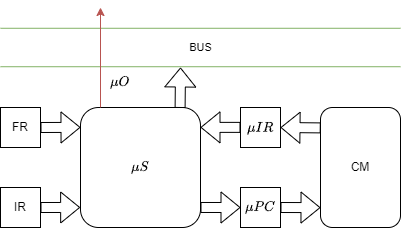
\includegraphics[width=0.8\textwidth]{media/mpcuarchitecture.png}
        \end{figure}
        \column{0.5\textwidth}
        \begin{itemize}
            \item \textbf{Control Memory $CM$}: Stores the microprogram (microinstructions).
            \item \textbf{Micro-Sequencer $\mu S$}: Fetches microinstructions from the control memory.
            \item \textbf{Micro-instruction Register $\mu IR$}: Stores the current microinstruction.
            \item \textbf{Micro-instruction Program Counter $\mu PC$}: Keeps track of the current microinstruction.
        \end{itemize}
    \end{columns}
    \note{
        The microprogrammed control unit consists of several key components:
        the control memory, micro-sequencer, micro-instruction register,
        and micro-instruction program counter.
        These components work together to fetch, store, and execute
        the microinstructions that generate control signals.
    }
\end{frame}

% Slide 7: Advantages of Microprogrammed Control Units
\begin{frame}
    \frametitle{Advantages of Microprogrammed Control Units}
    \begin{itemize}
        \item \textbf{Flexibility}: Easy to update; modifying control
        logic only requires updating the microprogram.
        \item \textbf{Simplicity}: Simplifies the design for CPUs
        with complex instruction sets.
        \item \textbf{Debugging}: Easier to debug because the logic is in the microcode.
        \item \textbf{Instruction Set Expansion}: Allows for adding new instructions
        \item \textbf{Less Hardware}: Requires less hardware than hardwired control units.
        \item \textbf{Emulates diffrent ISAs}: Can emulate any ISA.
    \end{itemize}
    \note{
        Microprogrammed control units are especially valuable in complex instruction
        set computers (CISC) due to their flexibility.
        Updating microinstructions is easier than changing hardware,
        which makes adding new instructions or optimizing existing ones simpler.
    }
\end{frame}

% Slide 7: Advantages of Microprogrammed Control Units
\begin{frame}
    \frametitle{Advantages of Microprogrammed Control Units}
    \begin{itemize}
        \item \textbf{Flexibility}: Easily updated by changing the microprogram.
        \item \textbf{Simplicity in Design}: Streamlines complex instruction set implementations.
        \item \textbf{Debugging Ease}: Centralized control logic simplifies error detection.
        \item \textbf{ISA Expansion}: Easily add new instructions.
        \item \textbf{Hardware Minimization}: Requires less control-specific hardware.
        \item \textbf{ISA Emulation}: Capable of emulating various instruction sets.
    \end{itemize}
    \note{
        Microprogrammed control units are highly flexible and easier to modify
        than hardwired units. This is especially beneficial in complex instruction
        set computers (CISC), where frequent updates are needed. Debugging is
        also simplified as the control logic is within the microprogram.
    }
\end{frame}

% Slide 8: Disadvantages of Microprogrammed Control Units
\begin{frame}
    \frametitle{Disadvantages of Microprogrammed Control Units}
    \begin{itemize}
        \item \textbf{Speed}: Slower than hardwired units due to microinstruction fetches.
        \item \textbf{Memory Requirements}: Additional memory required for microprogram storage.
    \end{itemize}
    \note{
        The primary downside of microprogrammed control units is their slower
        execution speed, as control signals must be fetched from memory.
        There's also memory overhead, as the microprogram must be stored
        separately from other data.
    }
\end{frame}

% Slide 9: Key Differences Between Control Units
\begin{frame}[fragile]
    \frametitle{Key Differences Between Control Units}
    \begin{table}
        \resizebox{0.9\textwidth}{!}{%
            \begin{tabular}{|c|c|c|c|}
                \hline
                \textbf{Feature} & \textbf{Unpipelined Hardwired} & \textbf{Microprogrammed} & \textbf{Pipelined Hardwired} \\
                \hline
                Control Signal Generation & Combinational Logic & Microinstructions & Combinational Logic \\
                \hline
                Flexibility & Low & High & Low \\
                \hline
                Best For & RISC & CISC & RISC/CISC \\
                \hline
                Memory Usage & No extra memory & Requires microprogram memory & Requires intermediate storage  \\
                \hline
                CPI & 1 & >1 & 1 \\
                \hline
                Cycle Time & Longer & Shorter (sequential) & Short (parallel)\\
                \hline
            \end{tabular}
        }
    \end{table}
    \note{
        This summary table contrasts each type of control unit across factors like flexibility,
        memory usage, and cycle time. Pipelined hardwired units,
        though similar to unpipelined ones in logic, can achieve lower cycle times
        due to parallelism.
    }
\end{frame}